% For TeXworks
\makeatletter
\declare@file@substitution{revtex4-1.cls}{revtex4-2.cls}
\makeatother

% Define document class
\documentclass[twocolumn,twocolappendix,linenumbers]{aastex631}

% \usepackage{showyourwork}
\usepackage{amsmath}
\usepackage{amssymb}
\usepackage{graphicx}
% \usepackage{layouts}
\usepackage{xcolor}
% \usepackage{upgreek}
\let\tablenum\relax
\usepackage{siunitx}
\usepackage{xspace}

% user-defined commands
% \newcommand{\yes}{\textcolor{green}{\checkmark}\xspace}
% \newcommand{\meh}{\textcolor{black}{$\sim$}\xspace}
% \newcommand{\no}{\textcolor{red}{$\times$}\xspace}
\newcommand{\osuaffil}{Department of Astronomy, The Ohio State University, 140 W. 18th Ave, Columbus OH 43210, USA}
\newcommand{\ccappaffil}{Center for Cosmology and AstroParticle Physics, The Ohio State University, 191 W. Woodruff Ave., Columbus OH 43210, USA}
\newcommand{\aFe}{[$\alpha$/Fe]\xspace}
\newcommand{\mathXH}{{\rm [X/H]}}
\newcommand{\mathOH}{{\rm [O/H]}}
\newcommand{\mathFeH}{{\rm [Fe/H]}}
\newcommand{\mathOFe}{{\rm [O/Fe]}}
\newcommand{\mathaFe}{{\rm [$\alpha$/Fe]}}
\newcommand{\yZ}[1]{$y/Z_\odot=#1$}
\newcommand{\vice}{{\tt VICE}\xspace}
% \newcommand{\hydro}{{\tt h277}\xspace}
\newcommand{\todo}[1]{{\color{red}#1}}

% Citation aliases
\defcitealias{johnson_stellar_2021}{J21}
\defcitealias{leung_variational_2023}{L23}
\defcitealias{dubay_galactic_2024}{D24}

\shorttitle{Two-Infall in VICE}
\shortauthors{Dubay et al.}
% \linespread{1.8}

\begin{document}

% Title
\title{Limitations on the Two-Infall Scenario in the Era of Large Stellar Age Catalogs}

% Author list
% \author[]{Amanda Ash}
\author[0000-0003-3781-0747]{Liam O.\ Dubay}
\affiliation{\osuaffil}
\affiliation{\ccappaffil}
\author[0000-0001-7258-1834]{Jennifer A.\ Johnson}
\affiliation{\osuaffil}
\affiliation{\ccappaffil}
\author[0000-0002-6534-8783]{James W.\ Johnson}
\affiliation{Observatories of the Carnegie Institution for Science, 813 Santa Barbara St., Pasadena CA 91101, USA}
% \affiliation{\osuaffil}
% \affiliation{\ccappaffil}
\author[0000-0002-2854-5796]{John D.\ Roberts}
\affiliation{\osuaffil}
\affiliation{\ccappaffil}
% \author[0000-0001-7775-7261]{David H. Weinberg}
\author{coauthors}

\correspondingauthor{Liam O.\ Dubay}
\email{dubay.11@osu.edu}

\begin{abstract}
    Stellar populations in the Milky Way exhibit a clear separation into two chemically distinct populations that are separated by their [$\alpha$/Fe] ratios. A popular explanation for this observation is the two-infall scenario, which postulates that two periods of substantial accretion rates dominate the assembly history of the Galaxy. However, most previous studies using the two-infall scenario have explored a limited portion of the parameter space, typically neglecting radial migration and assuming that the Galactic disk never ejected a substantial outflow. Thanks to advances in stellar age measurements in recent years, we can now also compare this popular model to more direct measurements of the Galaxy's evolutionary timescales from large stellar catalogs. We run multi-zone galactic chemical evolution (GCE) models with a two-infall-driven star formation history, radially dependent mass-loaded outflows, and a prescription for radial migration tuned to a hydrodynamic simulation. We compare our model results to abundance patterns across the disk from APOGEE DR17 and early data from the SDSS-V Milky Way Mapper program, supplemented with stellar age estimates through multiple methods. Although the two-infall scenario offers a natural explanation for the [$\alpha$/Fe] bimodality, it struggles to explain several features of the age--abundances structure in the disk. The two-infall scenario generically predicts a massive and long-lasting dilution event, but the data show that stellar metallicity is remarkably constant with age across much of the Galactic disk. This apparent age-independence places considerable restrictions upon the two-infall parameter space. These issues can be mitigated, but not completely resolved, by allowing the accreted gas to be pre-enriched to low metallicity.
\end{abstract}

% \section{Outline}
% \begin{enumerate}

    \item Introduction
    \begin{enumerate}
        \item Hook, summary of alpha-bimodality
        \item Summary of two-infall literature
        \item Summary of secular evolution models which claim alpha-bimodality
        \item Goal of the paper
    \end{enumerate}
    
    \item Methods
    \begin{enumerate}
        \item Description of GCE models
        \begin{enumerate}
            \item {\it Plot:} Two-infall parameters in one-zone models. The second infall timescale $\tau_2$ is the most important parameter for fitting the low-alpha sequence and the MDF.
        \end{enumerate}
        \item Motivate outflow prescription
        \item Discuss yields
        \begin{enumerate}
            \item {\it Plot:} Yield scaling in one-zone models. No yield set is fully compatible with the observed abundance history, so we investigate both the high yield and low yield cases in our multi-zone models.
        \end{enumerate}
        \item Describe data sources
    \end{enumerate}
    
    \item Multi-zone model results
    \begin{enumerate}
        \item Stellar abundance distributions
        \begin{enumerate}
            \item {\it Plot:} Stellar [O/Fe] distributions from multi-zone models with the low and high yield sets. Using the higher yields, the global [O/Fe] distribution is triple-peaked which does not fit the data.
            \item {\it Plot:} Abundance diagram from a high-yield one-zone model which illustrates that the turn-over in [O/Fe] evolution due to the second infall epoch produces an intermediate [O/Fe] peak in the stellar distribution.
        \end{enumerate}
        \item The radial abundance gradient
        \begin{enumerate}
            \item {\it Plot:} Radial abundance gradients predicted by multi-zone models with low and high yields.
            \item A variable second infall timescale
            \item Altering the outflow prescription
        \end{enumerate}
        \item Abundance histories
        \begin{enumerate}
            \item {\it Plot:} Comparison of stellar age-abundance diagrams from multi-zone models with low and high yields. The second infall epoch produces substantial dilution of the ISM metallicity, for which there is little observational evidence. Higher yields help the system recover from perturbations more rapidly and are in less disagreement with the data.
            \item {\it Plot:} Similar, but showing the mode of the stellar abundance distributions over time compared to the data. Due to the dilution from the second infall, the Solar neighborhood spends less time in equilibrium in the high-yield case, and doesn't yet reach equilibrium in the low-yield case.
            \item Can CGM pre-enrichment mitigate dilution and/or approach to equilibrium issues?
            \item Other parameters that can mitigate these issues
        \end{enumerate}
    \end{enumerate}
    
    \item Discussion
    \begin{enumerate}
        \item Other ways to fix the thin disk abundances
        \begin{enumerate}
            \item {\it Plot:} The DTD in one-zone models. A prompt DTD can reduce the size of the low-alpha loop, but it messes up the high-alpha sequence.
            \item {\it Plot:} Adjusting the thick-to-thin disk prescription in one-zone models. If the mass in the first infall is significantly more substantial, the [O/Fe] distribution better matches the data in the high yield case.
        \end{enumerate}
        \item Radial gas flows
        \item SF hiatus not driven by infall history
        \begin{enumerate}
            \item {\it Plot:} An SFE-driven hiatus in a one-zone model can produce alpha-bimodality without altering the gas inflow prescription.
        \end{enumerate}
    \end{enumerate}
    
    \item Conclusions
    \begin{enumerate}
        \item Summary of findings
        \begin{enumerate}
            \item Attempts to fix the problem with the [O/Fe] distribution in the thin disk end up creating issues with other observables, such as the thick/thin disk surface density ratio, the SN Ia DTD, or the age-metallicity relation.
            \item The equilibrium model, if accurate, places very strict limits on the two-infall model, moreso than for other models.
            \item A short ($\sim200$ Myr) star formation hiatus early in the history of the disk is sufficient to produce a bimodal distribution of [O/Fe] without altering the gas infall prescription. This is distinct from the star formation hiatus produced by the two-infall model.
        \end{enumerate}
    \end{enumerate}
\end{enumerate}

\section{Introduction}

% \todo{Hook, summary of alpha-bimodality.}
Studies of galactic chemical evolution (GCE) aim to explain observed stellar abundance patterns by modeling the star formation history of the Milky Way. A long-standing paradigm of GCE has been that the metallicity of the interstellar medium (ISM) increases over time due to supernova enrichment from successive generations of stars. In this view, one feature of the Milky Way disk that is difficult to explain is the so-called ``$\alpha$-bimodality'': the presence of two populations of stars at similar metallicity but separated by their \aFe ratio \citep[e.g.,][]{bensby_exploring_2014}. The high-$\alpha$ sequence consists of old stars \citep[$\sim9$ Gyr;][]{pinsonneault_apokasc-3_2025} with super-Solar \aFe and is associated with the kinematic thick disk \citep[e.g.,][]{fuhrmann_nearby_1998}, while the low-$\alpha$ sequence is younger, with approximately Solar \aFe, and is associated with the thin disk. The $\alpha$-bimodality is present across the Galactic disk, but the relative strength of the high- and low-$\alpha$ sequences varies by location \citep{hayden_chemical_2015}.

% Summary of two-infall literature
The two-infall model of chemical evolution was proposed by \citet{chiappini_chemical_1997} to explain the origin of the thick and thin disks. Though the model has been revised and refined since, the basic premise remains the same: the rate of gas infall onto the Galaxy is described by two consecutive, exponentially declining bursts. The relatively low infall rate between the two bursts leads to a hiatus in the star formation rate, allowing the gas abundance to evolve between the high- and low-$\alpha$ sequences without producing many stars in between. 
% By varying the timescale of the second infall, the model can produce inside-out disk growth and a radial abundance gradient.
The initial model of \citet{chiappini_chemical_1997} successfully reproduced the available abundance data at the time, which were largely confined to the Solar neighborhood.

Subsequent studies refined the two-infall model to reproduce abundance data across the disk \citep[e.g.,][]{chiappini_abundance_2001,chiappini_oxygen_2003}, and others have explored in its context the SN Ia delay-time distribution \citep{matteucci_effect_2009,palicio_analytic_2023}, galactic fountains \citep{spitoni_effects_2009}, radial gas flows \citep{spitoni_effects_2011,palla_chemical_2020}, a variable star formation efficiency \citep{spitoni_effects_2011,palla_chemical_2020}, radial stellar migration \citep{spitoni_effect_2015,palla_mgfe_2022}, azimuthal abundance variations due to spiral modes \citep{spitoni_2d_2019}, and pre-enriched gas infall \citep{palla_chemical_2020,spitoni_remind_2024}. Recently, \citet{spitoni_beyond_2023} and \citet{palla_mapping_2024} proposed a third gas accretion event in the last $\sim3$ Gyr to match the inferred star formation history from {\it Gaia} \citep{ruiz-lara_recurrent_2020} and explain the recent abundance evolution of the Solar neighborhood.

\todo{Observational evidence.} \citet{nissen_high-precision_2020} measured abundances and estimated ages for nearby Solar-type stars and reported two sequences in the age--metallicity distribution which could be explained by the two-infall model \todo{(rewrite)}. \citet{nataf_accurate_2024} also observe multiple sequences in the age--metallicity relation in their sample of $\sim400,000$ local subgiants, although the break between them is not as clean as in \citet{nissen_high-precision_2020}. \citet{chen_recent_2025} however argue that this trend can be explained by a smooth star formation history with inside-out growth: the older sequence consists of stars which have migrated from the inner galaxy, where the star formation rate peaked early, while the younger sequence was formed locally. 

\todo{Outflows.} Most previous studies of the two-infall model do not include mass-loaded outflows. Some hydrodynamic simulations of Galactic fountains ejected by CC SNe have shown that ejected material falls back onto the disk on relatively short timescales \citep{spitoni_galactic_2008,spitoni_effects_2009} and close to the point of origin \citep{melioli_hydrodynamical_2008,melioli_hydrodynamical_2009}, suggesting the effect on GCE could be minimal. However, other simulations of MW-like galaxies with different feedback prescriptions do produce mass-loaded outflows \todo{(citations)}. Empirically, mass-loaded outflows have been observed in nearby starburst galaxies \todo{(citations)} and dwarf galaxies \todo{(citations)} but not MW-like systems due to current detection limits \todo{(citations)}. We adopt an {\it ad hoc} prescription for outflows as a function of radius in order to balance different yield sets and reproduce the radial metallicity gradient.

\todo{Migration.} The two-infall model attempts to reproduce the full distribution of stellar abundances in the Solar neighborhood through a single, continuous evolutionary track. \todo{Talk about migration studies and why we don't need a single evolutionary track to explain the bimodality.}

\todo{Summary of secular evolution models which claim alpha-bimodality.} \citep{kubryk_evolution_2015}. \citep{sharma_chemical_2021} . \citep{chen_chemical_2023}.\citep{prantzos_origin_2023}.

\todo{Introduce equilibrium model.}

Recently, \citet{dubay_galactic_2024} studied the effect of the SN Ia delay-time distribution in the context of several different star formation histories, including a two-infall model. While the results did not greatly depend on the choice of SFH, the authors \todo{(we?)} noted that the two-infall model, as implemented, produced a stellar [O/Fe] distribution with three distinct peaks, at variance with the data.

\todo{Goal of paper.} 

\section{Observational Sample}
\label{sec:observational-sample}

\begin{table*}
    \centering
    \caption{Sample selection parameters and median uncertainties from APOGEE DR17 (see Section \ref{sec:observational-sample}).}
    \label{tab:sample}
    \begin{tabular}{lll}
        \hline\hline
        \multicolumn{1}{c}{Parameter} & \multicolumn{1}{c}{Range or Value} & \multicolumn{1}{c}{Notes} \\
        \hline
        $\log g$            & $1.0 < \log g < 3.8$          & Select giants only \\
        $T_{\rm eff}$       & $3500 < T_{\rm eff} < 5500$ K & Reliable temperature range \\
        $S/N$               & $S/N > 80$                    & Required for accurate stellar parameters \\
        ASPCAPFLAG Bits     & $\notin$ 23                   & Remove stars flagged as bad \\
        EXTRATARG Bits      & $\notin$ 0, 1, 2, 3, or 4     & Select main red star sample only \\
        Latent age          & $\sigma_\tau/\tau < 40\%$     & Age uncertainty from \citet{leung_variational_2023} \\
        $R_{\rm gal}$     & $3 < R_{\rm gal} < 15\,{\rm kpc}$    & Eliminate bulge \& extreme outer-disk stars \\
        $|z|$               & $|z| < 2\,{\rm kpc}$                 & Eliminate halo stars \\
        \hline
    \end{tabular}
\end{table*}

\begin{table*}
\centering
\caption{Number of APOGEE stars in each Galactic region.}
\label{tab:apogee-regions}
\begin{tabular}{r|cccccc}
\hline\hline
$R_{\rm gal}\in$ & $(3, 5]$ kpc & $(5, 7]$ kpc & $(7, 9]$ kpc & $(9, 11]$ kpc & $(11, 13]$ kpc & $(13, 15]$ kpc \\
$|z|\in$ &  &  &  &  &  &  \\
\hline
$(1.0, 2.0]$ kpc & 2013 & 2100 & 8734 & 3663 & 1324 & 363 \\
$(0.5, 1.0]$ kpc & 2487 & 3490 & 13811 & 9069 & 3289 & 460 \\
$(0.0, 0.5]$ kpc & 3296 & 7029 & 17319 & 16276 & 6336 & 812 \\
\hline
\end{tabular}

\end{table*}

\begin{table*}
    \centering
    \caption{Median and dispersion in APOGEE parameter uncertainties.}
    \label{tab:uncertainties}
    \begin{tabular}{lcc}
        \hline\hline
        \multicolumn{1}{c}{Parameter} & \multicolumn{1}{c}{Median Uncertainty} & \multicolumn{1}{c}{Uncertainty Dispersion ($95\%-5\%$)} \\
        \hline
        [Fe/H]          & $0.0089$   & $0.0060$ \\
        $\mathOFe$  & $0.019$    & $0.031$ \\
        $\log_{10}(\tau_{\rm latent}/{\rm Gyr})$    & 0.10   & $0.16$ \\
        $\tau_{\rm [C/N]}/{\rm Gyr}$     & 1.0   & \todo{N/A} \\
        \hline
    \end{tabular}
\end{table*}

We compare our models against stellar abundances from the Apache Point Observatory Galactic Evolution Experiment \citep[APOGEE;][]{majewski_apache_2017} data release 17 \citep[DR17;][]{abdurrouf_seventeenth_2022}. APOGEE data were obtained from infrared spectrographs \citep{wilson_apache_2019} mounted on the 2.5-meter Sloan Foundation Telescope \citep{gunn_25_2006} at Apache Point Observatory and the Ir{\'e}n{\'e}e DuPont Telescope \citep{bowen_optical_1973} at Las Campanas Observatory. The data reduction pipeline is described by \citet{nidever_data_2015}, and APOGEE Stellar Parameter and Chemical Abundance Pipeline (ASPCAP) is detailed by \citet{holtzman_abundances_2015}, \citet{garcia_perez_aspcap_2016}, and \citet{jonsson_apogee_2020}.

We obtain a sample of \num{171635} red giant branch and red clump stars with high-quality spectra using the selection criteria listed in Table \ref{tab:sample}, which are adapted from \citet{hayden_chemical_2015}. Table \ref{tab:uncertainties} presents the median statistical uncertainty and uncertainty dispersion ($95^{\rm th} - 5^{\rm th}$ percentile difference) of the calibrated [Fe/H] and [O/Fe] abundances for our sample. When calculating the galactocentric radius $R_{\rm gal}$ and midplane distance $z$ of each star, we use the \citet{bailer-jones_estimating_2021} photo-geometric distance estimates from {\it Gaia} Early Data Release 3 \citep{gaia_collaboration_gaia_2016,gaia_collaboration_gaia_2021} included in the APOGEE DR17 catalog and we adopt the Galactic coordinates of the Sun $(R,z)_\odot=(8.122, 0.0208)\,{\rm kpc}$ \citep{gravity_collaboration_detection_2018,bennett_vertical_2019}. Table \ref{tab:apogee-regions} presents the number of APOGEE stars in bins of $R_{\rm gal}$ and $|z|$; typical distance uncertainties are much smaller than the bin width.

We supplement the APOGEE DR17 abundance data with two different age catalogs. The first is the ``latent'' age estimates from \citet{leung_variational_2023}, who train a variational encoder-decoder network on asteroseismic data for APOGEE red giants. This catalog has two main advantages for our purposes: their method is designed to reduce contamination from abundance information (in particular [$\alpha$/Fe]), and the recovered ages do not plateau at $\sim10\,{\rm Gyr}$ as they do in some other neural network-derived age catalogs \citep[e.g.,][]{mackereth_dynamical_2019}. Following the recommendations of \citet{leung_variational_2023}, we use an upper limit on the relative age uncertainty of 40\%. This produces a sample of \num{57607} stars with latent age estimates, of which \num{14871} are in the Solar neighborhood ($7\leq R_{\rm gal}<9\,{\rm kpc}$, $0\leq|z|<0.5\,{\rm kpc}$). The median uncertainty in $\log({\rm age}/{\rm Gyr})$ is 0.10 (see Table \ref{tab:uncertainties}).

Our second age catalog uses the [C/N]--age relation for red giant branch and red clump stars. 
\todo{Paragraph describing [C/N]-derived ages (get help from Jack).}
This method has the benefit of providing age estimates for luminous giants, which increases the sample size at larger distances from the Sun. However, systematic effects of the [C/N]--age relation mean that these ages are most trustworthy in the range $1\sim10$ Gyr. We estimate ages for \num{113464} stars across the disk, including \num{20995} in the Solar neighborhood.
\todo{Note about metallicity cutoff for luminous giants.}

\section{Chemical Evolution Models \& Parameter Selection}
\label{sec:methods}

We run multi-zone GCE models using the Versatile Integrator for Chemical Evolution \citep[{\tt VICE};][]{johnson_impact_2020}. The basic format of our models follows \citet{johnson_stellar_2021} and \citet{dubay_galactic_2024}. We set up a disk with radial extent $0\leq R_{\rm gal}<20\,{\rm kpc}$ that is divided into concentric rings of width $\delta R_{\rm gal}=100\,{\rm pc}$. We use a time-step size of $\Delta t=10\,{\rm Myr}$ and a resolution of $n=8$ stellar populations per time-step per ring, and we run our models up to a final time of $t_{\rm final}=13.2\,{\rm Gyr}$.

Within each ring, chemical evolution proceeds according to a conventional one-zone GCE model with instantaneous mixing and continuous recycling. Stellar populations migrate between zones as described in Section \ref{sec:migration}, allowing the long-lived progenitors of SNe Ia to enrich areas of the Galaxy outside of their birth zones. We inhibit star formation past $R_{\rm gal}>15.5\,{\rm kpc}$, so stars in the outer 4.5 kpc of the model disk represent a purely migrated population. We also assign a final midplane distance to each stellar population as described in Section \ref{sec:migration}. We do not incorporate radial gas flows between the different zones, but we discuss their potential implications in Section \ref{sec:radial-flows}.

We discuss our assumptions about the nucleosynthetic yields in Section \ref{sec:yields}, and we detail our outflow prescription in Section \ref{sec:outflows}. We describe the gas supply in Section \ref{sec:sfh}, we detail the infall parameter selection in Section \ref{sec:parameter-selection}, and we present our star formation law in Section \ref{sec:sf-law}. We briefly summarize the stellar migration prescription in Section \ref{sec:migration}. Table \ref{tab:multizone-parameters} summarizes the most relevant variables and their fiducial values in this work.

\begin{deluxetable*}{Cccl}
    \tablecaption{A summary of variables and their fiducial values for our chemical evolution models (see discussion in Section \ref{sec:methods}).\label{tab:multizone-parameters}}
    \tablehead{
        \colhead{Quantity} & \colhead{Fiducial Value(s)} & \colhead{Section} & \colhead{Description}
    }
    \startdata
        % Yields
        % y/Z_\odot       & 1         & \ref{sec:yields}  & Nucleosynthetic yield scaling (see Table \ref{tab:yields}) \\
        % N_{\rm Ia}/M_\star  & $1.55\times10^{-3}$       & \ref{sec:yields}  & Integrated Type Ia supernova rate (see Table \ref{tab:yields}) \\
        f_{\rm Ia}(t)   & Equation \ref{eq:plateau-dtd}   & \ref{sec:yields}  & Delay-time distribution of Type Ia supernovae \\
        % t_D             & 40 Myr    & \ref{sec:yields}  & Minimum SN Ia delay time \\
        % Star formation histories
        % Outflows
        % \eta_\odot      & 0.2       & \ref{sec:outflows}    & Outflow mass-loading factor in the Solar annulus ($\eta\equiv \dot\Sigma_{\rm out}/\dot\Sigma_\star$) \\
        R_\eta          & 5.0 kpc   & \ref{sec:outflows}    & Exponential outflow scale radius \\
        f_{\Sigma,0}    & 0.27      & \ref{sec:sfh}     & Central thick/thin disk surface density ratio \\
        \mathXH_{\rm CGM}   & Pristine  & \ref{sec:sfh}     & Metallicity of infalling gas \\
        \tau_1          & 1 Gyr     & \ref{sec:parameter-selection}     & Timescale of the first infall epoch \\
        \tau_2(R_\odot)  & 15 Gyr    & \ref{sec:parameter-selection}     & Timescale of the second infall epoch at the Solar annulus \\
        R_{\tau_2}   & 7 kpc     & \ref{sec:parameter-selection}      & Exponential scale radius of the second infall timescale \\
        t_{\rm max}      & 4.2 Gyr  & \ref{sec:parameter-selection}     & Time of maximum gas infall (onset of second infall) \\
        \sigma_{\rm RM8}    & 2.68 kpc  & \ref{sec:migration}   & Radial migration strength
    \enddata
\end{deluxetable*}
\vspace{-24pt}

\subsection{Nucleosynthetic Yields}
\label{sec:yields}

\begin{table}
    \centering
    \caption{Nucleosynthetic yields and outflow prescriptions.}
    \begin{tabular}{c|ccc}
\hline\hline
 & $y/Z_\odot=1$ & $y/Z_\odot=2$ & $y/Z_\odot=3$ \\
\hline
$y_{\rm O}^{\rm CC}$ & \num{5.72e-03} & \num{1.14e-02} & \num{1.72e-02} \\
$y_{\rm Fe}^{\rm CC}$ & \num{4.58e-04} & \num{9.15e-04} & \num{1.37e-03} \\
$y_{\rm O}^{\rm Ia}$ & \num{0} & \num{0} & \num{0} \\
$y_{\rm Fe}^{\rm Ia}$ & \num{1.08e-03} & \num{1.83e-03} & \num{2.50e-03} \\
\hline
$N_{\rm Ia}/M_\star\,[{\rm M}_\odot^{-1}]$ & \num{1.55e-03} & \num{2.62e-03} & \num{3.57e-03} \\
$\eta_\odot$ & 0.2 & 1.4 & 2.4 \\
$R_\eta$ [kpc] & 4.2 & 5.4 & 7.2 \\
\hline
\end{tabular}

    \label{tab:yields}
\end{table}

The population-averaged nucleosynthetic yields of CCSNe are still fairly uncertain. This problem is exacerbated by the complexity of the CCSN explosion landscape \citep{sukhbold_core-collapse_2016}. Recently, \citet{weinberg_scale_2024} used a measurement of the mean Fe yield of CC SNe by \citet{rodriguez_iron_2023} and the plateau in stellar \aFe abundances at low metallicity to infer population-averaged yields of $y/Z_\odot\approx1$ --- in other words, the scale of SN yields is similar to the Solar abundance. However, \citet{johnson_milky_2024} found that GCE models with yields at this scale approach present-day abundances too slowly. We therefore investigate yield sets at multiple scales, which are presented in Table \ref{tab:yields}.

The SN Ia yield of Fe, $y_{\rm Fe}^{\rm Ia}$, is calculated so that the combined Fe yield $y_{\rm Fe}^{\rm Ia+CC}=y/Z_\odot$. We further increase $y_{\rm Fe}^{\rm Ia}$ by a factor of 30\% and 10\% for the \yZ{1} and \yZ{2} yield sets, respectively, to ensure that our models reach $\mathOFe\approx0.0$ by the end time. The fifth row of Table \ref{tab:yields} reports the integrated SN Ia rate $N_{\rm Ia}/M_\star$ from each yield set, assuming a mean Fe yield per SN Ia of $\overline m_{\rm Fe}^{\rm Ia}=0.7$ M$_\odot$ \citep{mazzali_common_2007,howell_effect_2009}. The rate for the \yZ{1} yield set is slightly higher than the volumetric rate of $N_{\rm Ia}/M_\star=(1.3\pm0.1)\times10^{-3}\,{\rm M}_\odot^{-1}$ reported by \citet{maoz_star_2017}, but is consistent with their measurement of $N_{\rm Ia}/M_\star=(1.6\pm0.3)\times10^{-3}\,{\rm M}_\odot^{-1}$ for field galaxies. The rate for the \yZ{2} yield set is consistent with the measurement of $N_{\rm Ia}/M_\star=(2.2\pm1.0)\times10^{-3}\,{\rm M}_\odot^{-1}$ by \citet{maoz_type-ia_2012}, while the rate for the \yZ{3} yield set is generally higher than literature values.

Unlike CCSNe, SNe Ia populate a broad distribution of delay times between progenitor formation and explosion. The time-dependent SN Ia rate in units of ${\rm M}_\odot^{-1}\,{\rm yr}^{-1}$ is defined as
\begin{equation}
    R_{\rm Ia}(t) = 
    \begin{cases}
        \frac{N_{\rm Ia}}{M_\star}
        \frac{f_{\rm Ia}(t)}{\int_{t_D}^{t_{\rm max}} f_{\rm Ia}(t') dt'}, & t \ge t_D \\
        0 & t < t_D,
    \end{cases}
    \label{eq:dtd-function}
\end{equation}
where $t_D=40\,{\rm Myr}$ is the minimum SN Ia delay time, $t_{\rm max}=13.2\,{\rm Gyr}$ is the lifetime of the disk, $N_{\rm Ia}/M_\star$ is the total number of SNe Ia per unit mass of star formation, and $f_{\rm Ia}(t)$ is the un-normalized form of the DTD. Motivated by the finding by \citet{dubay_galactic_2024} that a large fraction of long-delayed SNe Ia improves agreement with the Milky Way's high-$\alpha$ sequence, we adopt a wide plateau DTD of the form
\begin{equation}
    \label{eq:plateau-dtd}
    f_{\rm Ia}(t) =
    \begin{cases}
        1, & t < 1\,{\rm Gyr} \\
        (t/1\,{\rm Gyr})^{-1.1}, & t \ge 1\,{\rm Gyr}.
    \end{cases}
\end{equation}
We discuss the implications of using a different DTD in Section \ref{sec:abundance-distributions}.

\todo{I'd like to compare these yields to previous studies, but it's been very difficult to make that comparison. I'm unsure whether the \citet{francois_evolution_2004} yields are net or gross (probably gross since their baseline is \citet{woosley_evolution_1995}). I tried to implement their yield tables in VICE, but the chemical evolution tracks came out looking very wrong. Also, they use a weird IMF.} \citet{francois_evolution_2004} report that their models are insensitive to changes in the yield at a factor of 2 level.

\begin{figure}
    \centering
    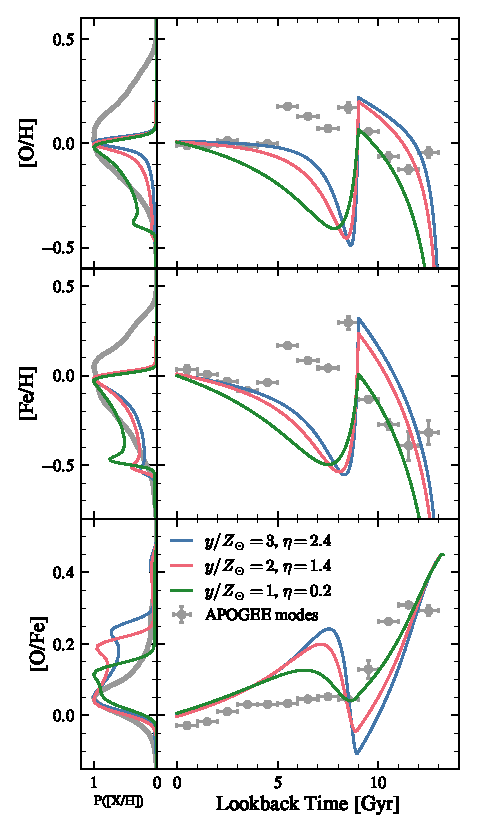
\includegraphics{figures/yield_outflow.pdf}
    \caption{The abundance evolution of three one-zone models with different yield and outflow settings. Table \ref{tab:yields} presents the population-averaged yields for each model. The gray points with error bars indicate the mode of the APOGEE abundance distributions from the Solar neighborhood ($7\leq R_{\rm gal}<9\,{\rm kpc}$, $0\leq|z|<0.5\,{\rm kpc}$) in 1 Gyr-wide bins of the \citet{leung_variational_2023} age estimates.}
    \label{fig:yield-outflow}
\end{figure}

Figure \ref{fig:yield-outflow} illustrates the effect of the yield scaling on the abundance evolution in one-zone models. All models feature a rapid dilution of the ISM metallicity by $\sim0.5-0.8$ dex, visible in the top two panels, brought on by the infall of pristine gas at $t_{\rm max}$. For the model with $y/Z_\odot=1$, this dilution persists for some time and the metallicity does not return to Solar until the present day. The models with higher yields and outflows recover from this dilution more quickly, returning to Solar metallicity by $\sim5\,{\rm Gyr}$ ago. However, the high-yield models experience a decline in [O/Fe] of $\sim0.2$ dex between the second infall and the present day, contrasted with the smaller decline of $\sim0.1$ dex in the low-yield model.

Figure \ref{fig:yield-outflow} also indicates the mode of the APOGEE abundance distributions in 1 Gyr-wide age bins. As explained by \citet{johnson_milky_2024}, the mode is expected to be less sensitive to the effects of radial migration than other statistical measures. The data show that the evolution in [O/H] is close to flat over the past 5 Gyr. The behavior of the $y/Z_\odot=2$ and $y/Z_\odot=3$ models closely matches this trend in the data, whereas the $y/Z_\odot=1$ model increases significantly by $\sim0.2$ dex during the same time period. The [Fe/H] abundance in the data does increase slightly at late times, likely due to the delayed contribution of Fe from SNe Ia. Between lookback times of $\sim5-9\,{\rm Gyr}$, the modes of [O/H] and [Fe/H] are higher than the present-day, likely due to a larger population of migrated stars relative to stars born in-situ at those times. 

The three models in Figure \ref{fig:yield-outflow} predict nearly identical evolution in [O/Fe] over the past 5 Gyr, and the trend in the data is similar apart from a $\sim0.05$ dex offset. \todo{Is this offset a problem? I could raise the SN Ia yields, but the global distributions would not match quite as well.} The offset between the data and models grows between $\sim5-8\,{\rm Gyr}$, especially for the higher yields. Of the three, the \yZ{2} and \yZ{3} models most closely match the observed late-time age--metallicity relations, whereas the \yZ{1} model shows the best agreement with the observed [O/Fe] evolution. As the $y/Z_\odot=2$ and $y/Z_\odot=3$ models show generally similar behavior, we focus on the $y/Z_\odot=1$ and $y/Z_\odot=2$ yield sets for the remainder of this work.

\subsection{Outflows}
\label{sec:outflows}

Most studies of the two-infall model assume the Milky Way has no significant mass-loaded outflows. Even in studies which do incorporate Galactic winds, the mass-loading is relatively weak \citep[e.g., $\eta\approx0.2$ in][]{palicio_analytic_2023}. To achieve a realistic radial metallicity gradient, many studies use a prescription for the infall timescale of the thin disk which increases linearly with radius \citep[e.g.,][]{chiappini_chemical_1997,romano_mass_2000}. Because we aim to study the effect of the yield assumptions on two-infall model predictions, we use mass-loaded outflows to control the final state of chemical evolution across the disk. As discussed by \citet{johnson_milky_2024}, evidence for or against outflows in Milky Way-type galaxies in simulations and observations is inconclusive.

\citet{weinberg_equilibrium_2017} showed that in the limit of continuous star formation, the ISM abundance approaches an equilibrium which is determined by the balance of yields, outflows, and star formation timescales. The mass-loading factor $\eta\equiv \dot\Sigma_{\rm out}/\dot\Sigma_\star$ required to reach equilibrium at Solar metallicity is
\begin{equation}
    \label{eq:equilibrium-eta}
    \eta_\odot = y_{\rm O}^{\rm CC} / Z_{\rm O,\odot} - 1 + r + \tau_\star / \tau_{\rm SFH},
\end{equation}
where $r=0.4$ is the instantaneous recycling parameter, $\tau_\star$ is the star formation efficiency timescale, and $\tau_{\rm SFH}$ is the star formation timescale. Equation \ref{eq:equilibrium-eta} informs our choice of $\eta$, but it is inaccurate in the two-infall case because of the bursty star formation history. Therefore, we tune the value of $\eta_\odot$ so that the model reaches $\mathOH=0.0$ by the end for each yield set, shown in Table \ref{tab:yields}.
% we find that if we adopt this prescription, models with $y/Z_\odot=1$ predict sub-Solar abundances at the present day because they have not yet reached their equilibrium value. 

We adopt a prescription for the outflow mass-loading factor which increases exponentially with radius:
\begin{equation}
    \eta(R_{\rm gal}) = \eta_\odot \exp\Big(\frac{R_{\rm gal}-R_\odot}{R_\eta}\Big)
\end{equation}
where $R_\eta$ is the exponential outflow scale radius and $R_\odot=8\,{\rm kpc}$. As discussed by \citet{johnson_milky_2024}, an exponential trend in $\eta$ with $R_{\rm gal}$ produces a linear trend in [Fe/H] with $R_{\rm gal}$. We adopt $R_\eta=5$ kpc, a lower value than in \citet{johnson_milky_2024}, so that our $y/Z_\odot=1$ model produces a radial abundance gradient of $\nabla\mathOH_{\rm eq}\approx-0.06\,{\rm dex}\,{\rm kpc}^{-1}$ \todo{(citations)}.
% The exponential outflow scale radius $R_\eta$ sets the equilibrium abundance gradient $\nabla\mathOH_{\rm eq}$:
% \begin{equation}
%     R_\eta = -\frac{1}{\nabla\mathOH_{\rm eq} \times\ln(10)}.
% \end{equation}
% We adopt $R_\eta=7.2\,{\rm kpc}$ as our fiducial value, which corresponds to $\nabla\mathOH_{\rm eq}=-0.06$ dex kpc$^{-1}$.
% \todo{Motivate exponential scale radius.}

\subsection{The Gas Supply}
\label{sec:sfh}

We run {\tt VICE} in ``infall mode,'' where we specify the gas infall density $\dot\Sigma_{\rm in}$ and the star formation effieciency (SFE) timescale $\tau_\star\equiv \Sigma_g / \dot\Sigma_\star$ as functions of time. The gas surface density $\Sigma_g$ and star formation rate $\dot\Sigma_\star$ are calculated from the two specified quantities according to our star formation law, which is described in Section \ref{sec:sf-law}, assuming zero initial gas mass in all zones.

The infall rate as a function of time and galactocentric radius can generically be described by
\begin{equation}
    \label{eq:infall-rate}
    \dot\Sigma_{\rm in}(t,R_{\rm gal}) = A f_{\rm in}(t|R_{\rm gal}) g(R_{\rm gal}),
\end{equation}
where $g(R_{\rm gal})=\Sigma_\star(R_{\rm gal}) / \Sigma_\star(R_{\rm gal}=0)$ is the stellar density gradient, $f_{\rm in}$ is the infall rate over time, and $A$ is the normalization. Because we incorporate mass-loaded outflows, $A$ is not analytically solvable, so first we numerically integrate the star formation rate $\dot\Sigma_\star(t,R_{\rm gal})$ and then follow the procedure outlined in Appendix B of \citet{johnson_stellar_2021} to calculate $A$. The infall rate is normalized to produce a total disk stellar mass of $(5.17\pm1.11)\times 10^{10}\,{\rm M}_\odot$ \citep{licquia_improved_2015} and to match the stellar surface density gradient of \citet{bland-hawthorn_galaxy_2016}.

The infall rate is described by two successive, exponentially declining bursts in time. The first infall component induces the formation of the thick disk, and the second component produces the thin disk. At a given galactocentric radius $R_{\rm gal}$, the un-normalized form of the infall rate is
\begin{equation}
    \label{eq:twoinfall-ifr}
    f_{\rm in}(t|R_{\rm gal}) = e^{-t/\tau_1} + f_{2/1}(R_{\rm gal}) e^{-(t-t_{\rm max})/\tau_2},
\end{equation}
where $\tau_1$ and $\tau_2$ are the first and second infall timescales, respectively, $t_{\rm max}$ is the onset of the second infall and thus the time of maximum gas infall, and $f_{2/1}$ is the ratio of the second infall amplitude to the first. We calculate $f_{2/1}$ for each zone such that the resulting stellar density profile follows a two-component disk, with the surface density ratio of the thick and thin disks given by
\begin{equation}
    f_\Sigma(R) \equiv \frac{\Sigma_1(R)}{\Sigma_2(R)} = f_{\Sigma,0} e^{R(1/R_2 - 1/R_1)}.
\end{equation}
We adopt a thick disk scale radius of $R_1=2.0\,{\rm kpc}$, a thin disk scale radius of $R_2=2.5\,{\rm kpc}$, and a central surface density ratio of $f_{\Sigma,0}=0.27$ \citep{bland-hawthorn_galaxy_2016}. \todo{Compare with other two-infall papers, which generally have a higher thick-to-thin ratio.}

In most of our models, we assume the infalling gas is pristine (i.e., $Z_{\rm in}=0$). However, the circumgalactic medium (CGM) from which the infalling gas is drawn could be previously enriched, either from gas stripped from dwarf galaxies or from SNe in the halo \todo{(citations; any measurements of CGM metallicity?)}. For this reason, we also test cases where the infalling gas is pre-enriched and its metallicity is described by
\begin{equation}
    \label{eq:pre-enrichment}
    Z_{\rm in}(t) = (1 - \exp(-t/\tau_{\rm rise})) Z_\odot 10^{\mathXH_{\rm CGM}}.
\end{equation}
In this case, the metallicity rises from 0 with a timescale $\tau_{\rm rise}=2\,{\rm Gyr}$ and plateaus at $\mathXH_{\rm CGM}=\mathOH_{\rm CGM}=\mathFeH_{\rm CGM}$. Previous GCE studies suggest that some level of enrichment of the infalling gas can improve agreement with observations \citep[e.g.,][]{palla_chemical_2020,johnson_milky_2024,spitoni_remind_2024}.
% We also investigate cases where the CGM is $\alpha$-enhanced, i.e., $\mathOFe_{\rm CGM}>0$.

\subsection{Infall Rate Parameter Selection}
\label{sec:parameter-selection}

\begin{figure*}
    \centering
    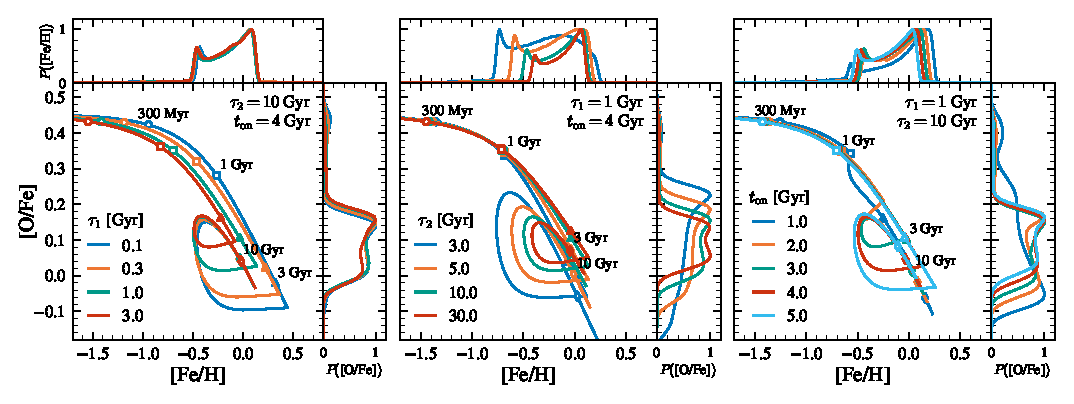
\includegraphics{figures/onezone_params.pdf}
    \caption{Gas abundance tracks in the [O/Fe]--[Fe/H] plane for one-zone chemical evolution models which assume different values for the infall history parameters. In each panel, one parameter is varied according to the legend while the other two are held fixed. The open symbols along each curve mark logarithmic steps in time, as denoted in panel (b). The marginal panels show the corresponding stellar abundance distributions, which are convolved with a Gaussian kernel with a width of 0.02 dex for visual clarity. All models use the \yZ{1} yield set and assume $\eta=0.2$.}
    \label{fig:twoinfall-parameters}
\end{figure*}

% The parameters of Equation \ref{eq:infall-rate} have important effects on the chemical evolution of the model. 
% Previous studies of the two-infall model have adopted values for the infall parameters of $\tau_1\sim0.1-1\,{\rm Gyr}$, $\tau_2\sim3-10\,{\rm Gyr}$, and $t_{\rm max}\sim3-5\,{\rm Gyr}$. 
Previous studies have adopted a wide range of parameters for Equation \ref{eq:twoinfall-ifr}. Figure \ref{fig:twoinfall-parameters} illustrates the effect of varying the infall parameters on gas abundance tracks and stellar abundance distributions in a one-zone model. The first infall timescale $\tau_1$, shown in panel (a), primarily affects the stellar distribution along the high-$\alpha$ sequence. Though $\tau_1$ has an apparently large effect on the size of the low-$\alpha$ loop, the effect on the stellar abundance distribution of the low-$\alpha$ sequence is quite small due to the low number of stars formed between $t\sim3-6\,{\rm Gyr}$. We adopt $\tau_1=1\,{\rm Gyr}$ for our fiducial value, in line with \citet{spitoni_galactic_2020} but longer than, e.g., \citet{nissen_high-precision_2020} or \citet{spitoni_apogee_2021}, in order to set the peak of the high-$\alpha$ sequence at $\mathOFe\approx+0.3$. 

Panel (b) of Figure \ref{fig:twoinfall-parameters} shows that 
% the second infall timescale $\tau_2$ is the most important parameter to tune in order to reproduce the observed stellar abundance distributions. 
the second infall timescale $\tau_2$ controls the width of the MDF and the low-$\alpha$ [O/Fe] distribution. A shorter $\tau_2$ produces a broader [O/Fe] distribution which is skewed to higher [O/Fe], while a longer $\tau_2$ produces both a narrower low-$\alpha$ sequence and a narrower MDF. We note that our maximum value of $\tau_2=30\,{\rm Gyr}$ is very close to a constant infall rate, so a further increase in $\tau_2$ has diminishing returns. Between $\tau_2=3-30\,{\rm Gyr}$, the endpoint of the abundance tracks shifts by $\sim0.2$ dex in [Fe/H] and $\sim0.1$ dex in [O/Fe], which could affect the model's ability to reproduce the present-day abundance of the Solar neighborhood. We adopt a fiducial value of $\tau_2=15\,{\rm Gyr}$ for the Solar neighborhood in order to minimize the width of the low-$\alpha$ [O/Fe] distribution while still approaching Solar [Fe/H] at late times. This value is in line with the infall timescale recovered by \citet{spitoni_galactic_2020}, and similar to the local star formation timescale adopted by \citet{johnson_stellar_2021}, but significantly longer than the timescales found by \citet{nissen_high-precision_2020} and \citet{spitoni_apogee_2021}. 
% In \todo{Section X}, we explore the effect of varying $\tau_2$ with radius in multi-zone models.

In our multi-zone models, we vary the second infall timescale with radius to produce inside-out growth of the disk. Previous multi-zone two-infall studies \citep[e.g.,][]{chiappini_abundance_2001,palla_chemical_2020} scale $\tau_2$ linearly with radius, with $\tau_2\approx1\,{\rm Gyr}$ in the inner disk and $\tau_2=7\,{\rm Gyr}$ at the Solar annulus. This prescription was adopted to match the metallicity distribution of the Solar neighborhood and the bulge in the absence of mass-loaded outflows \citep{romano_mass_2000}. We instead adopt an exponential $\tau_2 - R_{\rm gal}$ relation, with $\tau_2(R_\odot)=15\,{\rm Gyr}$ at the Solar annulus and a scale radius $R_{\tau_2}=7\,{\rm kpc}$. This is similar to the star formation history timescale of \citet{johnson_stellar_2021}, which was based on the  stellar age gradients in Milky Way-like spirals observed by \citet{sanchez_spatially_2020}. We also run models with a linear prescription and with a uniform value for $\tau_2$ and find little difference in our key results.

Finally, panel (c) of Figure \ref{fig:twoinfall-parameters} shows that the time of maximum infall $t_{\rm max}$ (c) strongly affects the overall stellar abundance distribution for values $t_{\rm max}\leq2\,{\rm Gyr}$, but in this case the gas tracks do not produce the characteristic abundance loop. For $t_{\rm max}>2\,{\rm Gyr}$, varying $t_{\rm max}$ results in a minor shift to the mean of the MDF and little change to the [O/Fe] distributions, even though the abundance tracks in [O/Fe]--[Fe/H] space appear very different. The value of $t_{\rm max}$ also slightly adjusts the ISM abundance endpoint, as a longer $t_{\rm max}$ means the chemical evolution ``reset'' from the second infall occurs closer to the present day (see discussion in Section \ref{sec:age-abundance}. We adopt a fiducial value of $t_{\rm max}=4.2\,{\rm Gyr}$ so that the second infall occurs at a lookback time of 9 Gyr, younger than the median age of the thick disk in the APOKASC-3 catalog of $9.14\pm0.05\,{\rm Gyr}$ \citep{pinsonneault_apokasc-3_2025}. This value is generally in line with previous two-infall studies \citep[e.g.,][]{nissen_high-precision_2020,spitoni_galactic_2020,spitoni_apogee_2021}.

We note that all our models are normalized to produce the same thick-to-thin-disk mass ratio of $f_{\Sigma,0}=0.27$ \citep{bland-hawthorn_galaxy_2016} at the Solar annulus regardless of the infall parameters. The high-$\alpha$ sequence appears much less prominent in our [O/Fe] distributions in Figure \ref{fig:twoinfall-parameters} than in the data because the model outputs include only stars which were formed in-situ at the Solar annulus. In our multi-zone models, most of the high-$\alpha$ stars present in the Solar neighborhood have migrated from the inner Galaxy.

\begin{figure*}
    \centering
    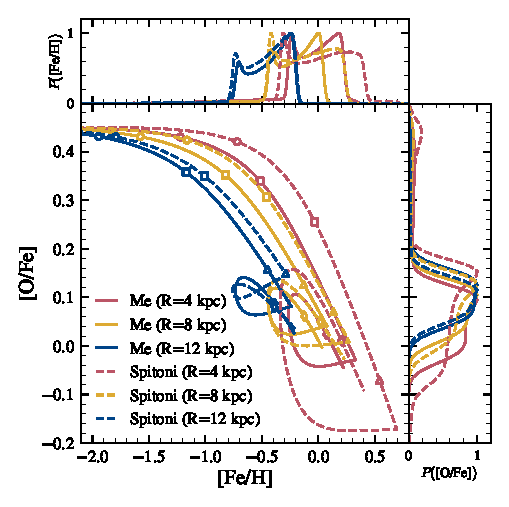
\includegraphics{figures/spitoni_comparison.pdf}
    \caption{Chemical abundance tracks and distributions from one-zone models which use our fiducial parameters (solid curves) and the MCMC-derived parameters from \citet[][dashed curves]{spitoni_apogee_2021}. All models use the $y/Z_\odot=1$ yield set. The time markers and marginal panels are the same as in Figure \ref{fig:twoinfall-parameters}. We also include a 2-D heatmap of the APOGEE stellar abundances in each panel for reference. APOGEE stars are restricted to (a) $2\leq R_{\rm gal}<6$ kpc, (b) $6\leq R_{\rm gal}<120$ kpc, and (c) $10\leq R_{\rm gal}<14$ kpc, and $0\leq |z|<2$ kpc in each panel. \todo{Should I instead compare to Palla et al. (2020), who have a more cohesive multi-zone model rather than three independent one-zone models?}}
    \label{fig:spitoni-comparison}
\end{figure*}

\todo{Highlight differences between our models and those of \citet{spitoni_apogee_2021} in Figure \ref{fig:spitoni-comparison}.} 

\subsection{The Star Formation Law}
\label{sec:sf-law}

The star formation law follows a single power-law prescription: $\dot\Sigma_\star\propto\Sigma_g^N$, with $N=1.5$ following \citet{kennicutt_global_1998}. Previous work with this GCE model \citep[e.g.,][]{johnson_stellar_2021,dubay_galactic_2024} assumed a three-component power-law, but we adopt a single power-law prescription in this work to allow for a more direct comparison with previous two-infall studies \citep[e.g.,][]{spitoni_remind_2024}. 

\begin{figure}
    \centering
    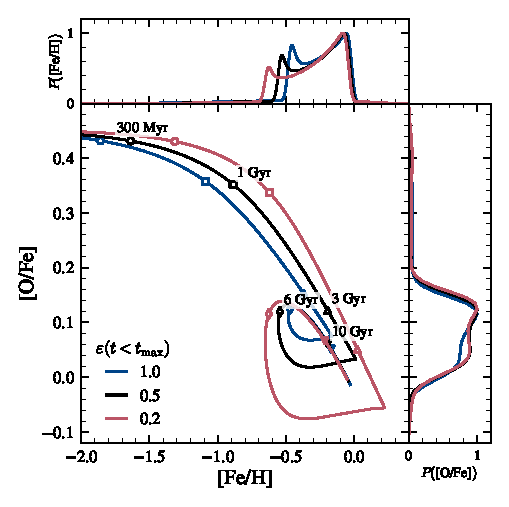
\includegraphics{src/tex/figures/sfe_prefactor.pdf}
    \caption{Effect of the SFE timescale pre-factor $\varepsilon$ on abundance tracks and distributions in a one-zone model (see Section \ref{sec:sf-law}). All models are normalized to produce roughly the same ratio of thick to thin disk stars regardless of the value of $\varepsilon$ during the first infall epoch.}
    \label{fig:sfe-prefactor}
\end{figure}

In detail, we calculate the star formation efficiency (SFE) timescale $\tau_\star\equiv\Sigma_g/\dot\Sigma_\star$ according to the following:
\begin{equation}
    \label{eq:sf-law}
    \tau_\star = 
    \begin{cases}
        \varepsilon(t) \tau_{\rm mol}(t),   & \Sigma_g \ge \Sigma_{g,0} \\
        \varepsilon(t) \tau_{\rm mol}(t) \Big(\frac{\Sigma_g}{\Sigma_{g,0}}\Big)^{-1/2}, & \Sigma_g < \Sigma_{g,0}
    \end{cases}
\end{equation}
where $\Sigma_{g,0} = 10^8\,{\rm M}_\odot\,{\rm kpc}^{-2}$ and $\tau_{\rm mol}(t)=\tau_{\rm mol,0}(t/t_0)^\gamma$, with $\gamma=1/2$, $t_0=13.8\,{\rm Gyr}$ \todo{(?)} and $\tau_{\rm mol,0}=2\,{\rm Gyr}$ \citet{leroy_star_2008}. Previous two-infall studies \citep[e.g.,][]{nissen_high-precision_2020} have adopted a higher SFE during the first infall epoch than during the second, which we emulate through the pre-factor $\varepsilon$:
\begin{equation}
    \label{eq:sfe-prefactor}
    \varepsilon(t) = 
    \begin{cases}
        0.5, & t < t_{\rm max} \\
        1.0, & t \ge t_{\rm max}.
    \end{cases}
\end{equation}
A lower value of $\varepsilon(t<t_{\rm max})$ leads to more efficient star formation during the first infall epoch. Figure \ref{fig:sfe-prefactor} illustrates that this pre-factor largely affects the metallicity of the high-$\alpha$ sequence, with a smaller $\varepsilon$ producing faster enrichment during the first infall and stronger dilution after $t_{\rm max}$. The pre-factor has virtually no effect on the overall [O/Fe] distribution because the model is normalized to produce the same thick-to-thin-disk mass ratio regardless of the details of the star formation law. We adopt $\varepsilon(t<t_{\rm max})=0.5$ for consistency with the two-infall literature. \todo{I actually think I can ditch the pre-factor, since the molecular timescale already decreases with lookback time. In fact, $\tau_{\rm mol}(4.2\,{\rm Gyr}) / \tau_{\rm mol}(13.2\,{\rm Gyr}) \approx 0.5$, which is pretty much the correct ratio to match the two-infall literature. The only catch is that $\tau_{\rm mol}$ is a very smooth transition, while with the prefactor it's an abrupt transition.}

\begin{figure}
    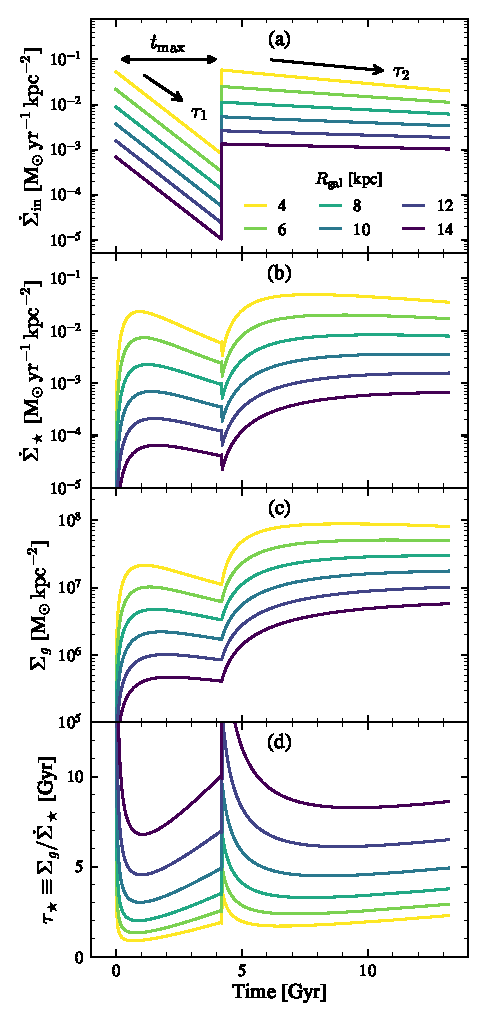
\includegraphics[width=\linewidth]{figures/star_formation_history.pdf}
    \caption{(a) The infall surface density, (b) the star formation surface density, (c) the gas surface density, and (d) the star formation efficiency timescale as a function of time for our fiducial multi-zone model with $y/Z_\odot=1$. Each panel plots the history for six different zones of width $\delta R_{\rm gal}=0.1\,{\rm kpc}$, color-coded by Galactocentric radius.}
    \label{fig:sfh}
\end{figure}

Figure \ref{fig:sfh} plots the star formation history of several different zones from our fiducial model with $y/Z_\odot=1$. In the inner Galaxy, the infall rate $\dot\Sigma_{\rm in}$ is similar at the start of the first and second infall epochs, and the star formation rate peaks at $t\approx7\,{\rm Gyr}$. In the outer Galaxy, the infall rate at $t_{\rm max}$ is significantly higher than at $t=0$, and the star formation rate is highest at the present day. The star formation efficiency timescale $\tau_\star$ spikes near $t=0$ and $t_{\rm max}$, but otherwise increases throughout the model's duration, reaching a maximum of $\tau_\star\approx2\,{\rm Gyr}$ in the inner disk and $\tau_\star\approx 9\,{\rm Gyr}$ in the outer disk.

\subsection{Stellar Migration}
\label{sec:migration}

This study is not the first to apply a prescription for radial migration to a two-infall GCE model. \citet{spitoni_effect_2015} explored the effect of migration speeds of order $\sim1\,{\rm km}{\rm s}^{-1}$ on the metallicity distribution of the Solar neighborhood. They prescribed some fraction of stars from the inner and outer Galaxy which contribute to the local present-day population based on a constant migration speed, and they also assumed some fraction of stars born in the Solar neighborhood will have migrated elsewhere. This method can improve agreement with the observed local metallicity distribution, but does not scale to abundance distributions across the disk. \citet{palla_mgfe_2022} compared the \citet{spitoni_effect_2015} prescription to the diffusion treatment of \citet{frankel_measuring_2018} and found similar results. Our implementation, described below, affects abundance distributions across the Galaxy, not just at the Solar annulus.

% \citet{spitoni_effect_2015} add a simple radial migration scheme to the model of \citet{spitoni_effects_2011}. They adopt stellar velocities of $\sim 1$ km s$^{-1}$ and assume that some fixed fraction of stars born at a given radius will end up in the Solar vicinity (10\% of those born at 4 kpc and 20\% at 6 kpc). This mimics the results of previous dynamical models such as \citet{minchev_chemodynamical_2013}. They find that by including stellar migration, they are better able to reproduce the high-metallicity tail of the local metallicity distribution, and they also argue that they constrain the migration speed to $0.5 < v < 2$ km s$^{-1}$ based on this tail. Their only point of comparison with data is the local G-dwarf metallicity distribution.

The distance a stellar population born at $R_{\rm form}$ migrates over its age $\tau$ is drawn from a Gaussian centered at 0 with standard deviation
\begin{equation}
    \sigma_{\rm RM} = \sigma_{\rm RM8} \Big(\frac{\tau}{8\,{\rm Gyr}}\Big)^{0.33} \Big(\frac{R_{\rm form}}{8\,{\rm kpc}}\Big)^{0.61},
    \label{eq:radial-migration}
\end{equation}
where we adopt $\sigma_{\rm RM8}=2.68\,{\rm kpc}$ as the fiducial value for the strength of radial migration. This is smaller than the value of $\sigma_{\rm RM8}=3.6\,{\rm kpc}$ found by \citet{frankel_measuring_2018}, but in Section \ref{sec:age-abundance} we explore the effect of a stronger migration prescription.

All stellar populations are born at the Galactic midplane and are assigned a final midplane distance $z$ drawn from the distribution
\begin{equation}
    p(z|\tau,R_{\rm final}) = \frac{1}{4 h_z} {\rm sech}^2\Big(\frac{z}{2 h_z}\Big),
    \label{eq:sech-pdf}
\end{equation}
where $R_{\rm final}$ is the final Galactocentric radius of the stellar population. The width of the distribution $h_z$ is given by
\begin{equation}
    h_z(\tau,R_{\rm final}) = \Big(\frac{0.24\,{\rm kpc}}{e^2}\Big) \exp\Big(\frac{\tau}{7\,{\rm Gyr}} + \frac{R_{\rm final}}{6\,{\rm kpc}}\Big).
    \label{eq:scale-height}
\end{equation}
We note that the final midplane distance is assigned at the end of the model run and therefore does not affect the chemical evolution.

The parameters of Equations \ref{eq:radial-migration} and \ref{eq:scale-height} were chosen to fit the stellar migration patterns in the {\tt h277} hydrodynamical simulation \citep{christensen_implementing_2012}. A more complete discussion of the migration scheme and its consequences can be found in Appendix C of \citet{dubay_galactic_2024}.

We note an important distinction between our method and that of \citet{spitoni_effect_2015}: SNe Ia from long-lived progenitors contribute Fe to each zone they migrate through, not just their birth zone. This is important because the median delay time of our SN Ia DTD is $\sim2$ Gyr, for which the width of the migration distribution is $\sigma_{\rm RM}\approx2$ kpc (Equation \ref{eq:radial-migration}). So, a significant fraction of SN Ia progenitors born in a given zone will enrich a disparate region of the Galaxy.

\section{Multi-Zone Model Results}
\label{sec:multizone-results}

\subsection{Local Abundance Patterns}
\label{sec:abundance-distributions}

\begin{figure}
    \centering
    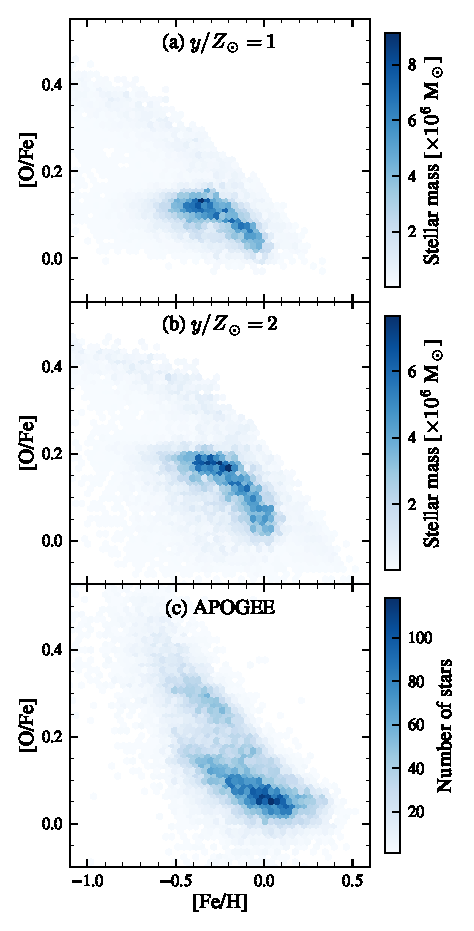
\includegraphics{figures/ofe_feh_density.pdf}
    \caption{The density of stars in the [O/Fe]--[Fe/H] plane from multi-zone models with (a) $y/Z_\odot=1$ and (b) $y/Z_\odot=2$, and (c) from the APOGEE DR17 catalog. The curves in panels (a) and (b) plot the ISM abundance of the Solar annulus over time, and the alternating black and white segments mark time intervals of {1 Gyr}. Stars are restricted to the region defined by $7\leq R_{\rm gal}< 9\,{\rm kpc}$ and $0.5\leq|z|<1\,{\rm kpc}$ to highlight the $\alpha$-bimodality.}
    \label{fig:ofe-feh-density}
\end{figure}

The two-infall model explains the chemical evolution of the thin disk through the low-$\alpha$ loop (see discussion in Section \ref{sec:parameter-selection}). However, inspection of the marginal [O/Fe] distributions in, e.g., Figure \ref{fig:yield-outflow} reveals a different morphology of the low-$\alpha$ sequence: the two-infall model predicts two peaks in [O/Fe] in the thin disk where the data show only one. The location of the second peak, at intermediate [O/Fe], varies depending on the yields (Figure \ref{fig:yield-outflow}) and infall parameters (Figure \ref{fig:twoinfall-parameters}), but is always present. This morphology remains essentially consistent in our multi-zone models as well, despite the inclusion of radial mixing and vertical dispersion of stars.

Figure \ref{fig:ofe-feh-density} illustrates the origin of the intermediate-$\alpha$ peak predicted by the two-infall model at mid to high Galactic latitudes. Between $0.5\leq|z|<1\,{\rm kpc}$, both the models with $y/Z_\odot=1$ and $y/Z_\odot=2$ predict an over-density of stars near the abundance turn-over ($\mathFeH\approx-0.3$, $\mathOFe\approx0.1-0.2$), which is not seen in the APOGEE sample. This over-density occurs because the overall rate of chemical evolution slows down $\sim2\,{\rm Gyr}$ after the second infall, and at the same time the delayed enrichment from SNe Ia reverses the evolution of [O/Fe]. This is a generic prediction of {\it any} two-infall model regardless of its specific parameters, though its impact can be mitigated through parameter choices which act to compress the distance between the low- and intermediate-$\alpha$ peaks, as in the $y/Z_\odot=1$ model in Figure \ref{fig:yield-outflow}.

Additionally, the shape of the low-$\alpha$ sequence in the model results (a concave-down ``comma'') is clearly different from the data (a concave-up ``swoosh''). \todo{Not sure what this means because the inside-out SFH has the same issue. Maybe it's related to radial migration?}

\subsection{Abundances Across the Disk}
\label{sec:disk-abundances}

\begin{figure*}
    \centering
    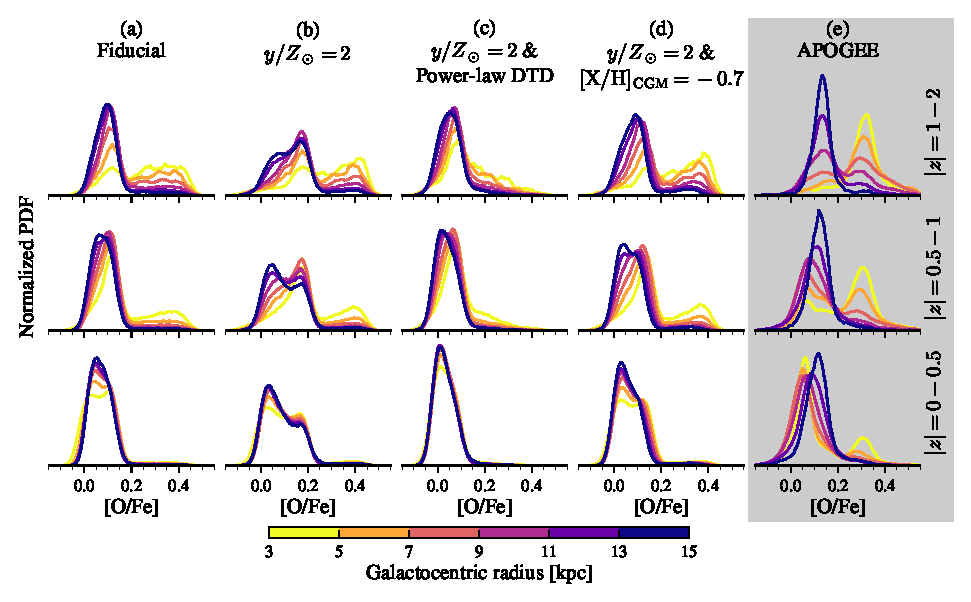
\includegraphics{src/tex/figures/ofe_df_comparison.pdf}
    \caption{Stellar [O/Fe] distributions produced by multi-zone models (a--d) and as observed by APOGEE (e). Stars are binned by Galactocentric radius, represented by the color scale, and absolute midplane distance $|z|$, represented by the different rows. Each distribution is normalized so that the area under the curve is 1, and the vertical scale is consistent across each row. The median APOGEE abundance uncertainties were forward-modeled onto the model outputs (see Table \ref{tab:uncertainties}). For visual clarity, each distribution is smoothed with a box-car of width 0.05 dex. Model (a) assumes the fiducial parameters and the \yZ{1} yield set, whereas models (b--d) assume the \yZ{2} yield set. Model (c) also assumes a power-law SN Ia DTD, while model (d) assumes the infalling gas has metallicity $\mathOH_{\rm CGM}=\mathFeH_{\rm CGM}=-0.7$. The distributions from APOGEE DR17 are plotted in column (e) for reference.}
    \label{fig:ofe-df}
\end{figure*}

The two-infall model generically predicts {\it three} peaks in the [O/Fe] distribution which correspond to the high-$\alpha$ sequence, the abundance ``turn-over'' after the second infall, and finally the late-time low-$\alpha$ sequence. Figure \ref{fig:ofe-df} compares [O/Fe] distributions across the Galactic disk produced by four different multi-zone models with the distributions observed in APOGEE DR17. For the fiducial model (a) with $y/Z_\odot=1$, the latter two peaks are close together and the overall effect is similar to the observed distribution. With a higher yield set, however, there is a $\sim0.2$ dex separation between the low- and intermediate-$\alpha$ peaks, because the CCSN element production after the second infall is more efficient. As a result, model (b) predicts a high density of stars in the APOGEE ``trough.''

In columns (c) and (d) of Figure \ref{fig:ofe-df}, we attempt to mitigate the issue of the intermediate-$\alpha$ peak for the $y/Z_\odot=2$ yield set. Model (c) switches out our fiducial DTD with a power-law DTD, which decreases the timescale for Fe production. However, as shown by \citet{dubay_galactic_2024}, models with a power-law DTD struggle to reproduce the high-$\alpha$ sequence for a wide range of star formation histories, and the results are no different for this two-infall model. 

Finally, in model (d) the metallicity of the infalling gas increases to $\mathXH_{\rm CGM}=-0.7$ at late times. We choose this value because it is the maximum which can plausibly still reproduce the disk abundances; any higher and the infalling gas would be more metal-rich than the most metal-poor thin disk stars. This model results in very similar [O/Fe] distributions to the $y/Z_\odot=1$ case. We assume that the infalling gas has $\mathOFe=0$ at all times; an alternate run with $\mathOFe=+0.3$ shifted the distribution towards higher [O/Fe], worsening agreement with observations. In summary, pre-enriched gas infall may be necessary for the two-infall model to match the observed [O/Fe] distribution across the disk.

\subsection{Local Abundance Evolution}
\label{sec:age-abundance}

\begin{figure*}
    \centering
    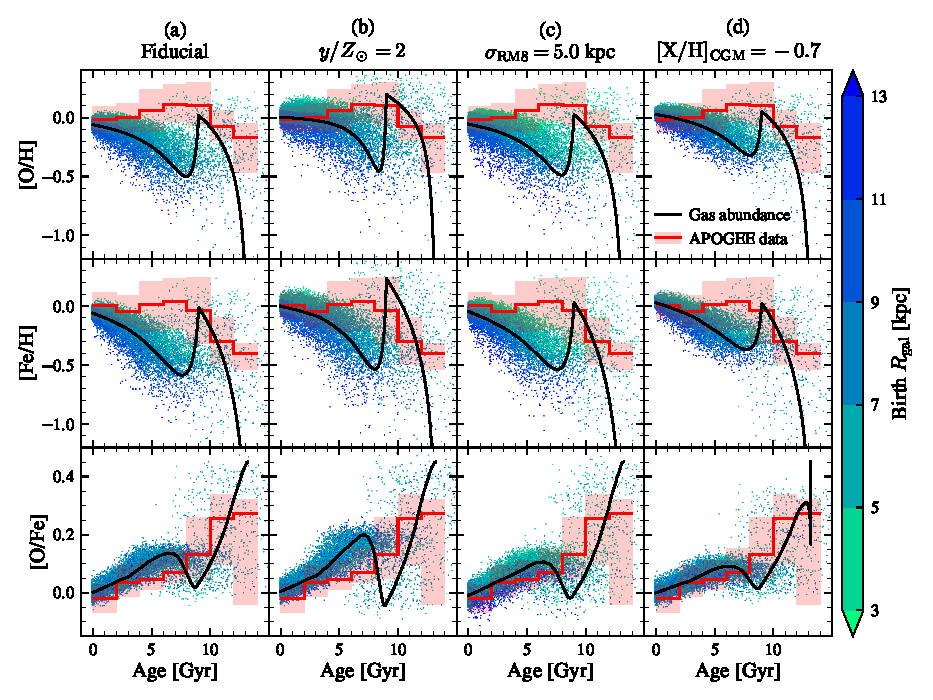
\includegraphics{figures/abundance_evolution.pdf}
    \caption{Stellar age--abundance relations produced by select multi-zone models. Each point represents a stellar population drawn from the Solar neighborhood near the midplane ($7\leq R_{\rm gal}\leq 9\,{\rm kpc}$, $0\leq |z| \leq 0.5\,{\rm kpc}$) and is color-coded by its birth radius. A Gaussian scatter has been applied to each point according to the median age and abundance uncertainties in Table \ref{tab:uncertainties}. For visual clarity, we plot a only random mass-weighted sample of \num{10000} points in each panel. The black curve plots the ISM abundance at $R_{\rm gal}=8\,{\rm kpc}$ over time. The red line segments plot the median abundance for APOGEE stars in {2 Gyr}-wide age bins, and the shaded regions represent the 16th--84th percentiles in each bin. Age estimates from APOGEE stars come from \citet{leung_variational_2023}. Each column shows results from a different multi-zone model: {\bf (a)} our fiducial model, with $y/Z_\odot=1$, $\sigma_{\rm RM8}=2.7\,{\rm kpc}$, and pristine gas infall; {\bf (b)} a model with higher yields $y/Z_\odot=2$; {\bf (c)} a model with greater radial migration strength $\sigma_{\rm RM8}=5\,{\rm kpc}$; and {\bf (d)} a model which assumes the infalling gas has metallicity $\mathOH_{\rm CGM}=\mathFeH_{\rm CGM}=-0.7$.}
    \label{fig:abundance-evolution}
\end{figure*}

The dilution effect discussed in Section \ref{sec:yields} is clearly seen in the multi-zone model results. Figure \ref{fig:abundance-evolution} shows stellar age--abundance relations for four model outputs. Column (a) plots the output of our fiducial model, with $y/Z_\odot=1$, $\sigma_{\rm RM8}=2.7\,{\rm kpc}$, and $Z_{\rm CGM}=0$. The fiducial model shows two major discrepancies with the \citet{leung_variational_2023} age--abundance relation: a major dilution of $\sim0.5$ dex at a lookback time of $\sim9\,{\rm Gyr}$ near where the data show a maximum in [O/H], and non-zero abundance evolution at late times where the data show very little abundance evolution. The evolution of [Fe/H] is similar, but the approach to Solar abundance is slower because of the additional delay imposed on Fe production from SNe Ia. A higher yield set (column b) mitigates both of these issues by shortening the time it takes the ISM metallicity to rebound post-$t_{\rm max}$, producing a much flatter abundance curve at late times. However, model (b) produces a poorer fit to the age--[O/Fe] relation; the decline in [O/Fe] over the thin disk epoch is much steeper than the data.

The observed rise in the median abundance of stars with ages of $\sim4-8\,{\rm Gyr}$ is thought to be due to radial migration, as those stars are more likely to have migrated from the dense inner metal-rich regions of the Galaxy during that time. Although our fiducial model does include a prescription for radial migration, the majority of stars in that age range in column (a) have sub-Solar abundances. Column (c) of Figure \ref{fig:abundance-evolution} presents a model with $y/Z_\odot=1$ but with a stronger migration prescription of $\sigma_{\rm RM8}=5\,{\rm kpc}$. Here, the stars which make up the present-day Solar neighborhood are drawn from a wider range of birth $R_{\rm gal}$, producing a broader abundance distribution for any given age. However, even though this prescription is much stronger than the estimates of, e.g., \citet{frankel_measuring_2018}, the model cannot reproduce the observed age--abundance trends in [O/H] and [Fe/H].

Finally, as in Section \ref{sec:abundance-distributions}, we investigate a model where the gas infall is pre-enriched to $\mathOH=\mathFeH=-0.7$. As shown in column (d) of Figure \ref{fig:abundance-evolution}, this mitigates but does not completely solve the two discrepancies. The dilution effect of the second infall is reduced to the $\sim0.3$-dex level as the gas which replenishes the Galaxy's reservoir is no longer pristine; however, the width of the stellar abundance distribution at any given age is also reduced, because the enriched gas accretion imposes a lower limit on the metallicity of the outermost regions, from which the stars of the low-metallicity tail in the Solar neighborhood are drawn. The late-time gas abundance evolution is similar to the fiducial model, but it ends at slightly super-Solar metallicity --- an effect which can be compensated by a slightly increased value of $\eta$. Overall, no modification to the $y/Z_\odot=1$ model is able to overcome both the dilution and late-time evolution issues.

\subsection{Abundance Evolution Across the Disk}
\label{sec:disk-evolution}

\begin{figure*}
    \centering
    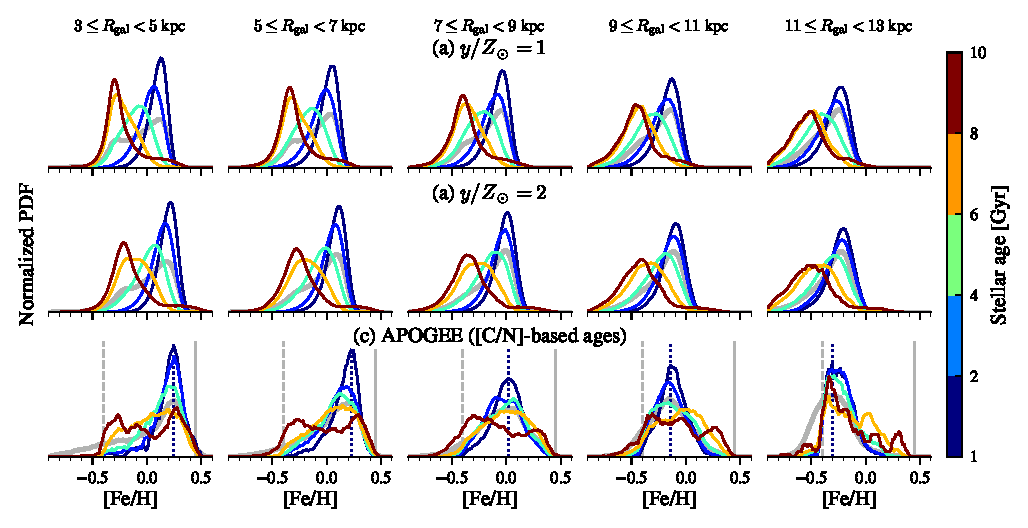
\includegraphics[width=0.9\linewidth]{figures/mdf_evolution.pdf}
    \caption{Evolution of the MDF across the Galactic disk. Each panel presents the normalized stellar [Fe/H] distribution within a {2 kpc}-wide annulus, color-coded by the age bin. Rows (a) and (b) present the distributions from multi-zone GCE models, while row (c) presents the distributions from APOGEE DR17 with ages derived from [C/N] abundances (see Section \ref{sec:observational-sample}). A Gaussian scatter has been applied to each model stellar population in rows (a) and (b) according to the median age and abundance uncertainties in Table \ref{tab:uncertainties}. The vertical blue dotted lines in row (c) mark the mode of the distribution in the $1-2\,{\rm kpc}$ age bin for reference. Also in row (c), the gray dashed line marks the cut at $\mathFeH>-0.4$ for upper red giant branch and red clump stars, and the gray solid line marks the cut at $\mathFeH<+0.45$ for all stars with [C/N]-based ages. Distributions in all panels are restricted to $0\leq|z|<0.5\,{\rm kpc}$ and boxcar-smoothed with a width of {0.1 dex}.}
    \label{fig:mdf-evolution}
\end{figure*}

The discrepancies between the predicted and observed abundance evolution discussed in Section \ref{sec:age-abundance} are also seen across the disk. Figure \ref{fig:mdf-evolution} shows the evolution of the MDF with age across five radial bins. We select the $y/Z_\odot=1$ and $y/Z_\odot=2$ models with pre-enriched infall due to the relative success of these models in the previous sections. We use the [C/N]-derived age estimates for the APOGEE sample due to the larger sample size in the most distant regions of the disk; we limit the comparison to ages $\leq10$ Gyr because of large systematic uncertainties for the oldest stars, as discussed in Section \ref{sec:observational-sample}. The two-infall model predicts a very broad MDF for ages $>10$ Gyr because of the rapid enrichment of the ISM during the first infall epoch.

Figure \ref{fig:mdf-evolution} shows that even with pre-enriched infall, both of our models predict that the MDF shifts to the left going from younger to older populations. On the other hand, the data show that the MDF broadens with age, which we attribute to radial migration, but its peak does not shift substantially over the past $\sim6-8$ Gyr. While the mode of the MDF shifts depending on the radial bin, its evolution is remarkably consistent over the entire disk, in line with the equilibrium scenario of \citet{johnson_milky_2024}.
\todo{Note about metallicity cutoff for luminous giants.}

On the other hand, the model predictions for the MDF in the $8-10\,{\rm Gyr}$ age bin are strikingly similar to the APOGEE MDF. The two-infall model predicts a bimodal distribution: the metal-rich component comprises stars formed during the last Gyr of the first infall epoch, and the metal-poor component is stars formed during the first Gyr of the second infall epoch (post-dilution). The data show this same bimodal structure in all but the outermost radial bin, with peaks at $\mathFeH\approx-0.3$ and $+0.3$. While the location of the model peaks depends on $R_{\rm gal}$, in the data they are quite consistent from the innermost to the outermost bin. \todo{I actually think the two-infall model gets this right for the wrong reasons. In the data, the left peak is the high-$\alpha$ sequence and the right is the high-metallicity end of the low-$\alpha$ sequence. In the model, the {\it right} peak is produced during the first infall (i.e., thick disk) and the {\it left} is immediately after the second infall (i.e., low-metallicity end of thin disk).}

\section{Discussion}
\label{sec:discussion}

\todo{Summary of problem: the two-infall model is boxed in by data.}

% \subsection{The SN Ia Delay-Time Distribution}
% \label{sec:dtd-discussion}

% \begin{figure*}
%     \centering
%     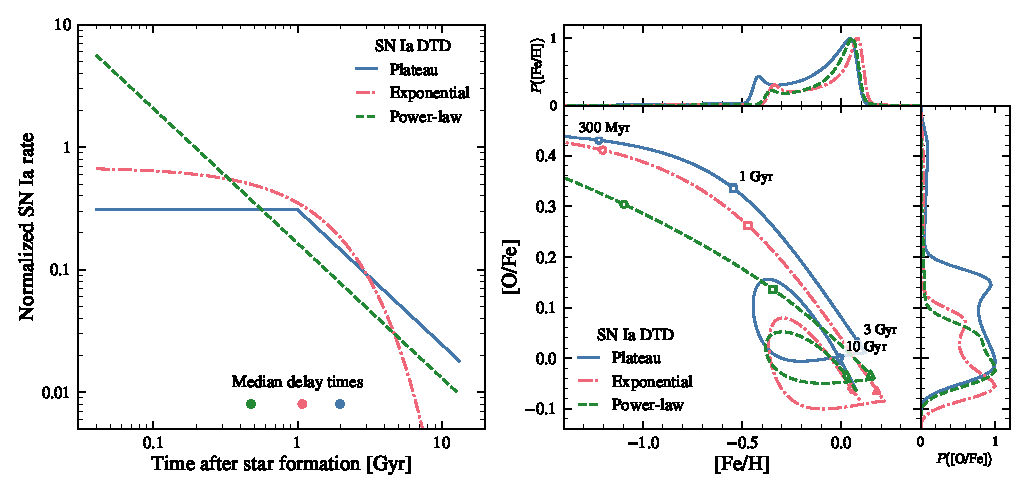
\includegraphics{figures/delay_time_distribution.pdf}
%     \caption{The effect of the SN Ia delay-time distribution (DTD) on chemical abundance tracks and stellar distributions. {\it Left:} The relative SN Ia rate as a function of time after star formation for each DTD model. The points illustrate the median delay times for each DTD. {\it Right:} Output of one-zone models which assume different SN Ia DTDs with the {\tt yZ2} yield set. The infall parameters are fixed at $\tau_1=1\,{\rm Gyr}$, $\tau_2=10\,{\rm Gyr}$, and $\tau_{\rm on}=3\,{\rm Gyr}$. {\bf Key takeaway:} the extent of the low-$\alpha$ sequence can be reduced by a more prompt SN Ia DTD, but the high-$\alpha$ sequence is also shifted to a more metal-poor regime.}
%     \label{fig:dtd}
% \end{figure*}

% Figure \ref{fig:dtd} illustrates the effect of the SN Ia DTD on the abundance predictions by the two-infall model. The fiducial plateau DTD produces the strongest high-$\alpha$ peak as well as the greatest separation between the two low-$\alpha$ peaks. The exponential DTD produces the most stars near Solar [O/Fe], but the low-$\alpha$ sequence is still distinctly bimodal. Finally, the power-law DTD shrinks the low-$\alpha$ loop such that there is only one low-$\alpha$ peak; however, this DTD produces high-$\alpha$ stars at metallicities much lower than observed, as discussed in \citet{dubay_galactic_2024}.

\subsection{Radial Gas Flows}
\label{sec:radial-flows}

\todo{Radial gas flows are hard :'(}

Some two-infall studies \citep[e.g.,][]{spitoni_effects_2011,palla_chemical_2020,palla_mapping_2024} implement inward radial gas flows with velocity $\sim1$ km s$^{-1}$ in order to reproduce the radial abundance gradient without Galactic outflows.

\citet{spitoni_effects_2011} find that a two-infall model of the disk without gas exchange produces a radial metallicity gradient which is too shallow. They implement an inward radial gas flow on the order of $\sim0-4$ km s$^{-1}$ which varies with radius, and find that it improves agreement with the observed gradient. However, they found that a variable star formation efficiency with radius in combination with a gas density threshold for star formation could also reproduce the observed gradient without radial flows.

\subsection{Star Formation Hiatus}
\label{sec:sfe-hiatus}

\begin{figure}
    \centering
    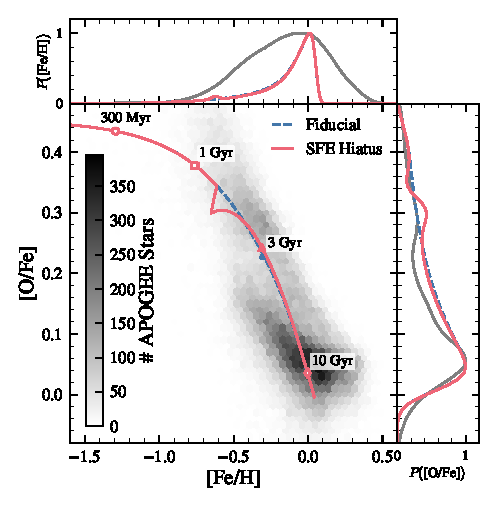
\includegraphics{figures/onezone_sfe_hiatus.pdf}
    \caption{Abundance tracks and distributions from one-zone models which experience an efficiency-driven starburst. The blue dashed curve represents the fiducial model that has an exponentially declining infall rate and constant star formation efficiency timescale $\tau_\star=2\,{\rm Gyr}$. The red solid curve plots the output of a model which experiences an enhancement of $\tau_\star$ by a factor of 10, for a duration of 200 Myr, starting at $t=1.4\,{\rm Gyr}$. Both models assume the \yZ{2} yield set, with $y_{\rm Fe}^{\rm Ia}$ reduced by 20\% to better match the model endpoint with the data, and $\eta=1.4$. The greyscale histogram presents the number density of APOGEE stars in the Solar annulus ($7\leq R_{\rm gal}\leq 9\,{\rm kpc}$, $0\leq|z|\leq2\,{\rm kpc}$) in [O/Fe]--[Fe/H] space, and the gray histograms in the marginal panels show the APOGEE stellar abundance distributions.}
    \label{fig:onezone-sfe-hiatus}
\end{figure}

The two-infall model falls into the broader category of GCE models which reproduce the $\alpha$-bimodality by halting or severely limiting star formation for some duration. For the two-infall model, this phase of low star formation immediately precedes the second infall epoch and is due to the relatively short timescale of the first infall epoch. However, as we have shown, the dilution of the ISM resulting from the second infall poses a challenge when comparing to age--abundance data.

A bursty infall history is not the only way to produce a gap in the star formation history. \citet{beane_rising_2024} present a simulated galaxy from the Illustris TNG50 suite that exhibits MW-like bimodality. They argue that the $\alpha$-bimodality is brought on by a brief ($\sim300\,{\rm Myr}$) quiescent period caused by bar formation. The virial mass of their galaxy grows steadily throughout this period, unlike in our two-infall model where the mass grows by a factor of \todo{X} during the 1 Gyr following the second infall.

While our semi-analytic model does not include a Galactic bar, we can explore the effects of a star formation hiatus by artificially boosting the SFE timescale $\tau_\star$ for a period of time. Figure \ref{fig:onezone-sfe-hiatus} illustrates the effect of this SFE-driven hiatus in a one-zone model with an exponentially declining infall rate. During the quiescent period, the [O/Fe] ratio slowly declines due to the delayed contribution of Fe from SNe Ia. Meanwhile, the gas mass continues to increase even as star formation is suppressed. When $\tau_\star$ is lowered at the end of the quiescent period, the high gas mass sparks a moderate star formation burst which causes stellar abundances to ``pile up'' at similar [O/Fe] values. The trough between the high- and low-$\alpha$ sequences results from the star formation returning to pre-quiescence behavior.

Our simple hiatus model offers a few parameters which control the chemical evolution. The onset time of the SFE hiatus controls the position of the high-$\alpha$ sequence: a later onset places the peak at lower [O/Fe]. The duration of the star formation hiatus \todo{(and the $\tau_\star$ enhancement factor?)} controls the strength of the high-$\alpha$ peak.

The parameters of the SFE hiatus in Figure \ref{fig:onezone-sfe-hiatus} were chosen to match the APOGEE stellar [O/Fe] distribution as closely as possible. However, there are some differences in detail, such as the dearth of stars at $\mathOFe\approx+0.35$ due to the star formation hiatus. We intend this model to illustrate another path to reproducing the $\alpha$-bimodality. Most of the high-$\alpha$ stars present in the Solar annulus have likely migrated from the inner Galaxy, where perhaps this SFE-driven hiatus was concentrated.

\section{Conclusions}
\label{sec:conclusions}

\begin{itemize}
    \item The ``turn-over'' in the evolution of [O/Fe] following the second infall produces a low-$\alpha$ sequence with a fundamentally different abundance structure than observed. A low yield set ($y/Z_\odot=1$) coupled with lower outflows, or pre-enrichment of the infalling gas, can bring the stellar [O/Fe] distributions more in line with the data.
    \item The large quantity of pristine gas accreted in the Solar neighborhood during the second infall phase rapidly dilutes the ISM metallicity by $\sim0.5$ dex. Models with a low yield set ($y/Z_\odot=1$) remain at sub-Solar metallicity until the present day, in stark contrast to the observed local age--metallicity relation. This issue can be mitigated with higher yields and outflows, but not by pre-enriched infall or radial migration.
    \item Our models predict that the MDF evolves to higher metallicity over time throughout the disk. This contrasts with the APOGEE data, which show very little change in the mode over the past $\sim6-8$ Gyr.
    \item The equilibrium scenario of chemical evolution, if correct, places stricter limits on the two-infall model than other evolutionary models.
\end{itemize}

\section*{Acknowledgements}

\todo{Personal acknowledgements.}

LOD and JAJ acknowledge support from National Science Foundation grant no.\ AST-2307621. JAJ and JWJ acknowledge support from National Science Foundation grant no.\ AST-1909841.
LOD acknowledges financial support from an Ohio State University Fellowship.
JWJ acknowledges financial support from an Ohio State University Presidential Fellowship and a Carnegie Theoretical Astrophysics Center postdoctoral fellowship. \todo{Update grants and fellowships.}

Funding for the Sloan Digital Sky 
Survey IV has been provided by the 
Alfred P.\ Sloan Foundation, the U.S.\ 
Department of Energy Office of 
Science, and the Participating 
Institutions. 

SDSS-IV acknowledges support and 
resources from the Center for High 
Performance Computing  at the 
University of Utah. The SDSS 
website is \url{www.sdss4.org}.

SDSS-IV is managed by the 
Astrophysical Research Consortium 
for the Participating Institutions 
of the SDSS Collaboration including 
the Brazilian Participation Group, 
the Carnegie Institution for Science, 
Carnegie Mellon University, Center for 
Astrophysics | Harvard \& 
Smithsonian, the Chilean Participation 
Group, the French Participation Group, 
Instituto de Astrof\'isica de 
Canarias, The Johns Hopkins 
University, Kavli Institute for the 
Physics and Mathematics of the 
Universe (IPMU) / University of 
Tokyo, the Korean Participation Group, 
Lawrence Berkeley National Laboratory, 
Leibniz Institut f\"ur Astrophysik 
Potsdam (AIP),  Max-Planck-Institut 
f\"ur Astronomie (MPIA Heidelberg), 
Max-Planck-Institut f\"ur 
Astrophysik (MPA Garching), 
Max-Planck-Institut f\"ur 
Extraterrestrische Physik (MPE), 
National Astronomical Observatories of 
China, New Mexico State University, 
New York University, University of 
Notre Dame, Observat\'ario 
Nacional / MCTI, The Ohio State 
University, Pennsylvania State 
University, Shanghai 
Astronomical Observatory, United 
Kingdom Participation Group, 
Universidad Nacional Aut\'onoma 
de M\'exico, University of Arizona, 
University of Colorado Boulder, 
University of Oxford, University of 
Portsmouth, University of Utah, 
University of Virginia, University 
of Washington, University of 
Wisconsin, Vanderbilt University, 
and Yale University.

This work has made use of data from the European Space Agency (ESA) mission
{\it Gaia} (\url{https://www.cosmos.esa.int/gaia}), processed by the {\it Gaia}
Data Processing and Analysis Consortium (DPAC,
\url{https://www.cosmos.esa.int/web/gaia/dpac/consortium}). Funding for the DPAC
has been provided by national institutions, in particular the institutions
participating in the {\it Gaia} Multilateral Agreement.

% From the Center for Belonging and Social Change, https://cbsc.osu.edu/about-us/land-acknowledgement
We would like to acknowledge the land that The Ohio State University occupies is the ancestral and contemporary territory of the Shawnee, Potawatomi, Delaware, Miami, Peoria, Seneca, Wyandotte, Ojibwe and many other Indigenous peoples. Specifically, the university resides on land ceded in the 1795 Treaty of Greeneville and the forced removal of tribes through the Indian Removal Act of 1830. As a land grant institution, we want to honor the resiliency of these tribal nations and recognize the historical contexts that has and continues to affect the Indigenous peoples of this land.

\software{\vice \citep{johnson_impact_2020}, Astropy \citep{astropy_collaboration_astropy_2013,astropy_collaboration_astropy_2018,astropy_collaboration_astropy_2022}, scikit-learn \citep{pedregosa_scikit-learn_2011}, SciPy \citep{virtanen_scipy_2020}, Matplotlib \citep{hunter_matplotlib_2007}.}

\appendix

\section{Reproducibility}
\label{app:reproducibility}

\todo{Blah.}

\bibliography{references}

\end{document}
